% CVPR 2022 Paper Template
% based on the CVPR template provided by Ming-Ming Cheng (https://github.com/MCG-NKU/CVPR_Template)
% modified and extended by Stefan Roth (stefan.roth@NOSPAMtu-darmstadt.de)

\documentclass[10pt,twocolumn,letterpaper]{article}

%%%%%%%%% PAPER TYPE  - PLEASE UPDATE FOR FINAL VERSION
%\usepackage[review]{cvpr}      % To produce the REVIEW version
\usepackage{cvpr}              % To produce the CAMERA-READY version
%\usepackage[pagenumbers]{cvpr} % To force page numbers, e.g. for an arXiv version

% Include other packages here, before hyperref.
\usepackage{graphicx}
\usepackage{amsmath}
\usepackage{amssymb}
\usepackage{booktabs}


% It is strongly recommended to use hyperref, especially for the review version.
% hyperref with option pagebackref eases the reviewers' job.
% Please disable hyperref *only* if you encounter grave issues, e.g. with the
% file validation for the camera-ready version.
%
% If you comment hyperref and then uncomment it, you should delete
% ReviewTempalte.aux before re-running LaTeX.
% (Or just hit 'q' on the first LaTeX run, let it finish, and you
%  should be clear).
\usepackage[pagebackref,breaklinks,colorlinks]{hyperref}


% Support for easy cross-referencing
\usepackage[capitalize]{cleveref}
\crefname{section}{Sec.}{Secs.}
\Crefname{section}{Section}{Sections}
\Crefname{table}{Table}{Tables}
\crefname{table}{Tab.}{Tabs.}


%%%%%%%%% PAPER ID  - PLEASE UPDATE
\def\cvprPaperID{*****} % *** Enter the CVPR Paper ID here
\def\confName{CVPR}
\def\confYear{2022}

\begin{document}

%%%%%%%%% TITLE - PLEASE UPDATE
\title{Egocentric Vision Project - MLDL Course}

\author{Andrea Cucchietti\\
Politecnico di Torino, Italy\\
{\tt\small s327134@studenti.polito.it}
% For a paper whose authors are all at the same institution,
% omit the following lines up until the closing ``}''.
% Additional authors and addresses can be added with ``\and'',
% just like the second author.
% To save space, use either the email address or home page, not both
\and
Annalisa Belloni\\
Politecnico di Torino, Italy\\
{\tt\small s330705@studenti.polito.it}
\and
Davide Elio Stefano Demicheli\\
Politecnico di Torino, Italy\\
{\tt\small s331531@studenti.polito.it}
}
\maketitle

%%%%%%%%% ABSTRACT
\begin{abstract}
    This work aims to delve into the domain of egocentric vision and its integration with Natural Language, in order to achieve video understanding. In particular, we focus our attention on the NLQ task of the Episodic Memory benchmark proposed by Ego4D, leveraging the VSLBase and VSLNet models.  
    Various configurations of these two models are tested, analyzing the effects of different choices of visual and text encoders, and
    the respective outcomes are presented in detail.  
    Furthermore, we propose to pre-train the best performing configuration on an LLM-generated dataset of queries. This approach leads to better performance after fine-tuning on the original benchmark data.
\end{abstract}

%%%%%%%%% BODY TEXT
\section{Introduction}
\label{sec:intro}

Egocentric Vision captures human interactions from a unique perspective, using cameras mounted directly on the user's head as they perform various actions. The release of large-scale datasets has advanced the frontier of first-person perception, encouraging the research community to explore new methods for learning from egocentric videos, such as using natural language queries for video understanding.\\
A big step forward was taken with the introduction of the Ego4D dataset: the world's largest first-person video ML dataset and benchmark suite \cite{grauman2022ego4d}.
The dataset contains 3,670 hours of densely narrated daily-life activity videos and a great number of annotations associated with five benchmark tasks.

Among these, we focused on the Episodic Memory benchmark, which aims to make past first-person visual experiences queryable. To be precise, given an egocentric video and a query, the Ego4D Episodic Memory task consists in pinpointing where the answer can be found within a long video.

In particular, the queries we address are natural language queries (NLQ), meaning each query is expressed in text (e.g., “What did I put in the drawer?”), and the relative output response is the temporal window where the answer is inferable, capturing the essence of Natural Language Video Localization (NLVL).
Being a vision-language understanding task, NLVL requires both computer vision and natural language processing techniques, leading us to adopt a cross-modal reasoning approach.

Inspired by the improvements of visual-textual embeddings and query-localization models, we tried to face one of the most relevant issues of the NLQ task: the limited number and scope of annotations, which is reflected in difficulties for the existing methods in learning about concepts that are poorly represented in training, for instance when we have complex queries addressing interactions between several visual entities.
This restricted quantity of annotations is due to the significant efforts that they require to be created. However, the dataset also includes narrations, another useful source of textual information for the videos, which are not only considerably easier to annotate but also more varied, significantly more numerous, and can be adapted to be employed for the NLQ task.

Specifically, we propose leveraging timestamped narrations to pre-train query-localization models. By utilizing a large language model (LLM) to automatically generate queries from these narrations, we aim to augment the existing dataset, providing more varied examples of queries, thereby improving the performance of query-localization models. This approach not only capitalizes on the abundance of narration data but also reduces the manual effort involved in query annotation, paving the way for more efficient and scalable data augmentation methods in wearable camera video analysis.

\begin{figure}[t]
   \centering
   
\includegraphics[width=1\linewidth]{images/merged_image_with_description_large_font.pdf}
   \caption{An example of NLQ task with query and relative temporal response window.}
   \label{fig:nlq_task}
\end{figure}
 
\section{Related Work}
The field of egocentric vision has seen significant advancements over the past few years. In this section, we review the most relevant literature, focusing our attention on the NLQ task and briefly outlining the context, the existing approaches, and the building blocks on which our work is based.
\subsection{Natural language video localization}
NLQ is a video grounding task in the Ego4D episodic memory benchmark which consists of temporally localizing where the answer of a natural language query can be seen in an egocentric video. 
Already existing video grounding methods like 2D-TAN \cite{zhang2020learning2dtemporaladjacent} and VSLNet \cite{zhang2020spanbasedlocalizingnetworknatural} have subsequently been adapted to handle this new task.

In particular, 2D Temporal Adjacent Network (2D-TAN) is a single-shot framework for moment localization, able to encode the adjacent temporal relations while learning discriminative features for matching video 
moments with the corresponding expressions. Its core idea is to retrieve a moment on a two-dimensional 
temporal map, which considers adjacent moment candidates as the temporal context.

VSLNet, instead, solves the NLVL task with a multimodal span-based QA framework, employing a query
guided highlighting (QGH) strategy which highlights the region where the model has to search.

Our objective, similarly to what has been done by Naq \cite{ramakrishnan2023naqleveragingnarrationsqueries}, is to further enhance these methods by 
employing data augmentation with narrations-based queries. The densely annotated narrations available in 
the EGO4D dataset are exploited as an additional and more general data source to improve the model’s 
ability to perform the NLQ task. This is realized by adapting and converting the narrations and their 
timestamps into NLQ annotations.  
However, while Naq employs the same narrations as queries (exploiting encoders that can effectively adapt 
to the difference between declarative sentences and questions), we instructed an LLM to generate the 
queries for the dataset augmentation.
\subsection{Text Encoders}
There are several approaches to the problem of text encoding. Two relevant examples are BERT \cite{devlin2019bert} and GloVe \cite{pennington-etal-2014-glove}.
These two language embedding models both fulfill the function of transforming textual input into vector representations. However, they present significantly different structures, which affect their characteristics and performance. The major difference between the two models is that GloVe is a static word embedding model: each word has a single representation vector that does not change, regardless of the context in which the word appears. In contrast, BERT is a contextual embedding model with a representation of each word that is dynamic and changes depending on the context.\\
The BERT embedding model learns word representations based on both preceding and following contexts (bidirectional) and is based on the Transformer architecture.\\
Given these two different natures, the GloVe-based text encoder is typically simpler and less computationally intensive, whereas the BERT-based encoder is more complex, requiring greater computational power, but also more powerful in the understanding.\\
We separately employed these two types of encoders within the VSLNet model to test and compare the results obtained with each approach.

\subsection{Vision Encoders}
Training models end-to-end on video datasets is often impractical due to the large computational budgets 
and time required. A common strategy adopted to bypass this problem is to leverage pre-trained models 
and fine-tune them for the specific downstream task we need to solve. Among these pre-trained models, 
we focused our attention on Omnivore \cite{girdhar2022omnivoresinglemodelvisual} and EgoVLP \cite{lin2022egocentricvideolanguagepretraining}.

Omnivore is a vision transformer model designed to handle multiple types of visual inputs such as images, 
videos, and 3D data with a single model architecture. The key idea behind Omnivore is to unify these 
different types of visual data representations into a common framework, allowing the final embeddings to be used for a wide variety of vision tasks. It utilizes a vision transformer architecture, which has proven effective in 
capturing long-range dependencies and contextual information in visual data. Pre-training on large, diverse 
datasets allows Omnivore to learn robust and general features that can be transferred to specific tasks, as in our case.

EgoVLP, instead, is a framework for video-language pre-training specifically tailored for egocentric video 
data. It addresses the challenges posed by unstructured and noisy data in the Ego4D dataset by curating a
pre-training dataset called EgoClip. Furthermore, the model’s ability to align video and textual representations is obtained using a contrastive learning approach exploiting the weak supervision of free
form textual narrations.

\subsection{LLM}
\textit{Gemma-2b-it-V2} \cite{gemmateam2024gemma} is part of a family of lightweight, state-of-the-art open models released by Google in 2024. The model has already been trained on a large dataset of textual data and serves as a valid and versatile tool for a wide range of natural language processing tasks. Further specialization in a particular task is possible by performing fine-tuning on that specific task.
Specifically, we used the \textit{Gemma-2b-it-V2} model, since it provides results of acceptable quality without requiring considerable computational resources.

\begin{figure}[h]
   \centering
   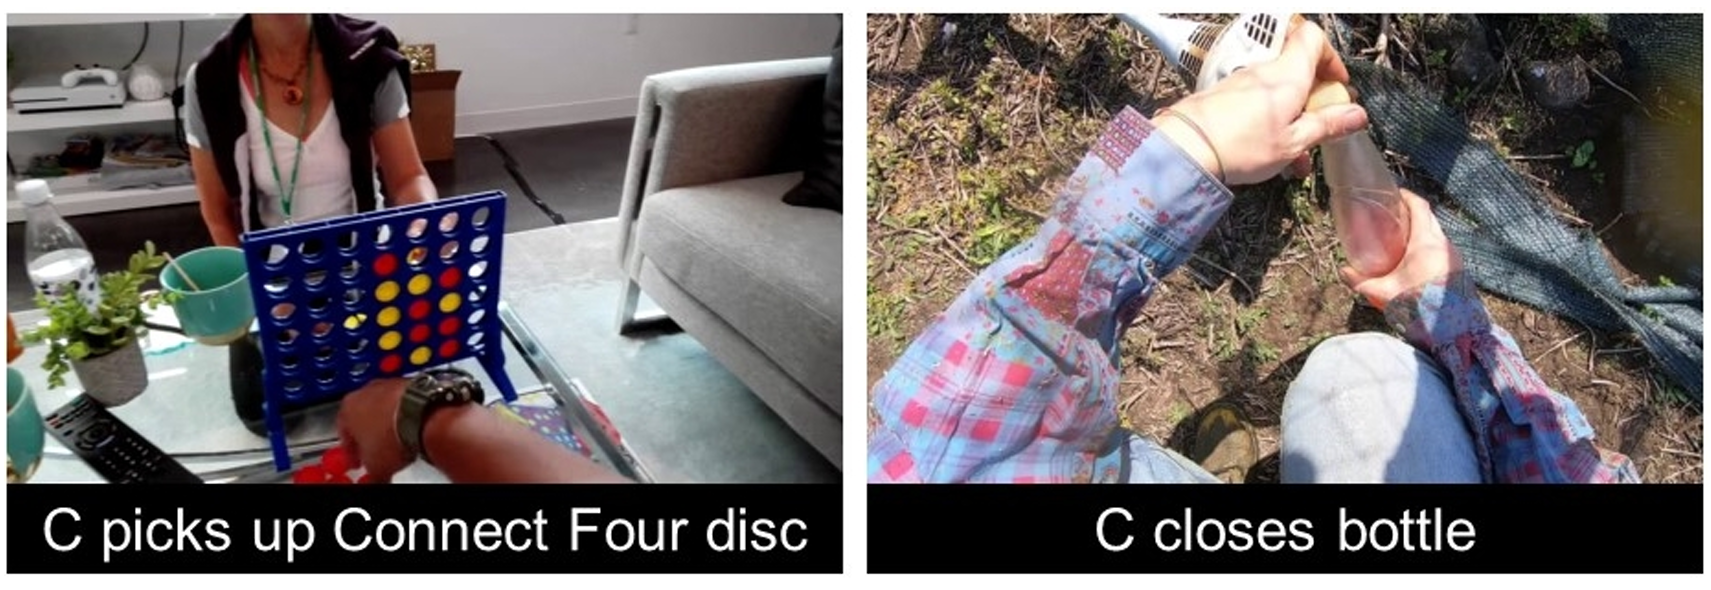
\includegraphics[width=1\linewidth]{images/2_images_with_narrations.png}
   \caption{Example of narrations. The letter C indicates the camera wearer.}
   \label{fig:nlq_task}
\end{figure}


\section{Dataset}
We will provide here a brief analysis of the Ego4D dataset that we used for our work. First, we will examine the annotations, which convey information related to the textual queries. For the NLQ-type queries related to the Episodic Memory benchmark, we have three files available: nlq\_train.json, nlq\_val.json, and nlq\_test\_unannotated.json. These files contain the portions of the dataset designated for the training, validation, and testing phases of the model, respectively. Each file includes a list of queries associated with information about the clip and the reference video. The first two files also provide the ground truth, represented by the start and end times of the response segment.

It should be noted that the following analyses were conducted on both the training and validation datasets, yielding conceptually analogous and consistent results. For brevity, we will refer only to the nlq\_train.json file, but similar observations apply to the validation set.

We then extended our preliminary analysis to the ego4d.json file, which contains metadata for the entire dataset, specifically linking each video to various scenarios.

The NLQ annotations are quite heterogeneous: they contain a large variety of queries and videos with different characteristics. The queries can be classified into 13 distinct templates that give the general structure for specific questions (e.g., “Did I leave the window open?” falls under the template “What is the state of object X?”). These templates are further grouped into three categories: \textit{Object}, \textit{People}, and \textit{Place}.

We conducted several analyses, available at \url{https://github.com/Cucchi01/episodic-memory/tree/nlq_fixes_and_fp16_support} in the branch \textbf{nlq\_fixes\_and\_fp16\_support} of the GitHub repository, but we report here only the most relevant ones for brevity.  \\
One of them, in particular, aimed to study the duration of the response segments independently of the template type, to determine the most frequent duration range in the dataset.
From \cref{fig:5}, it is evident that most response segments have a relatively short duration, typically falling below \(100\) frames, which corresponds to approximately \(3.5\) seconds.

\begin{figure}[h]
    \centering
    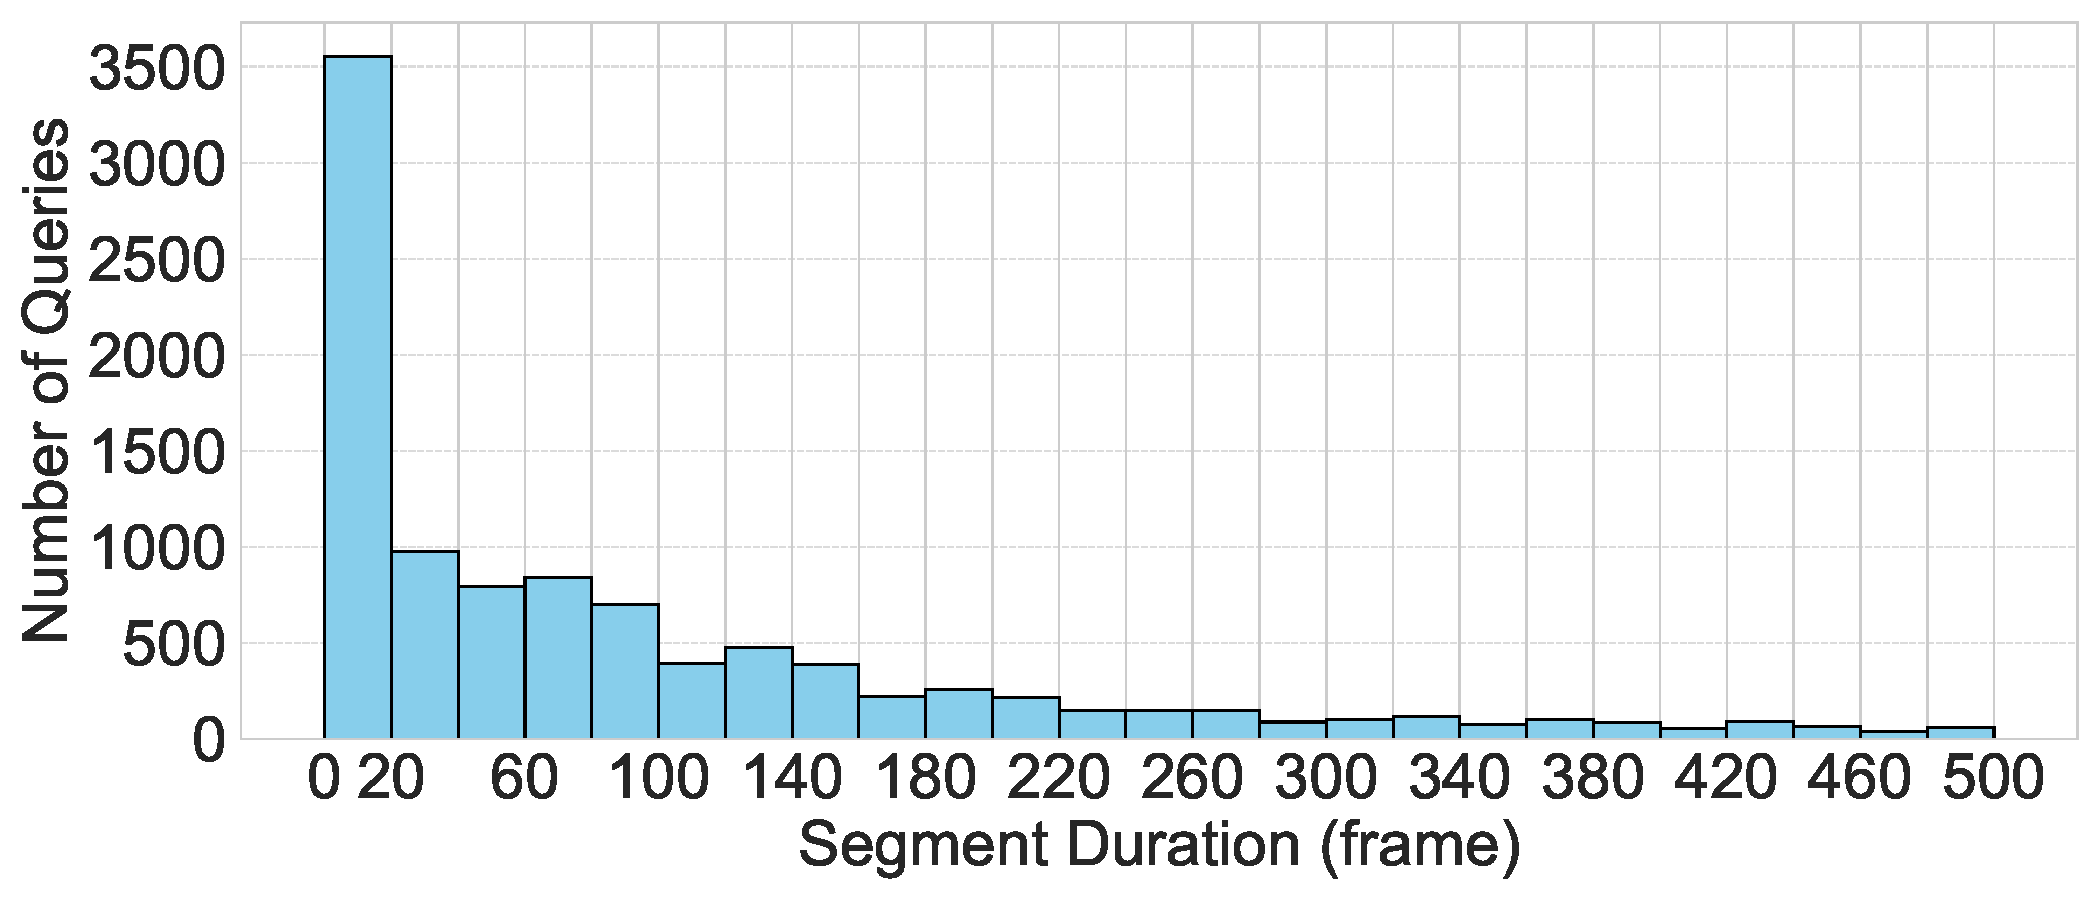
\includegraphics[width=1\linewidth]{images/NumberQueriesByResponseDuration_large_font.pdf}
    \caption{Number of Queries by Response-Segment Duration.}
    \label{fig:5}
\end{figure}

Then, we studied the distribution of the response segments throughout the reference clip to understand which section of the clip had the highest concentration of questions and answers. To achieve this, we assigned a rational number between 0 and 1 to each query, indicating the relative position of the response segment's midpoint within the clip. Subsequently, we computed the number of queries in the dataset that were located close to the same relative position in their respective clips.\\
By looking at \cref{fig:6}, we can clearly notice how most queries are located towards the beginning and end of the reference clip, with fewer occurrences in the central zone. 

\begin{figure}[t]
    \centering
    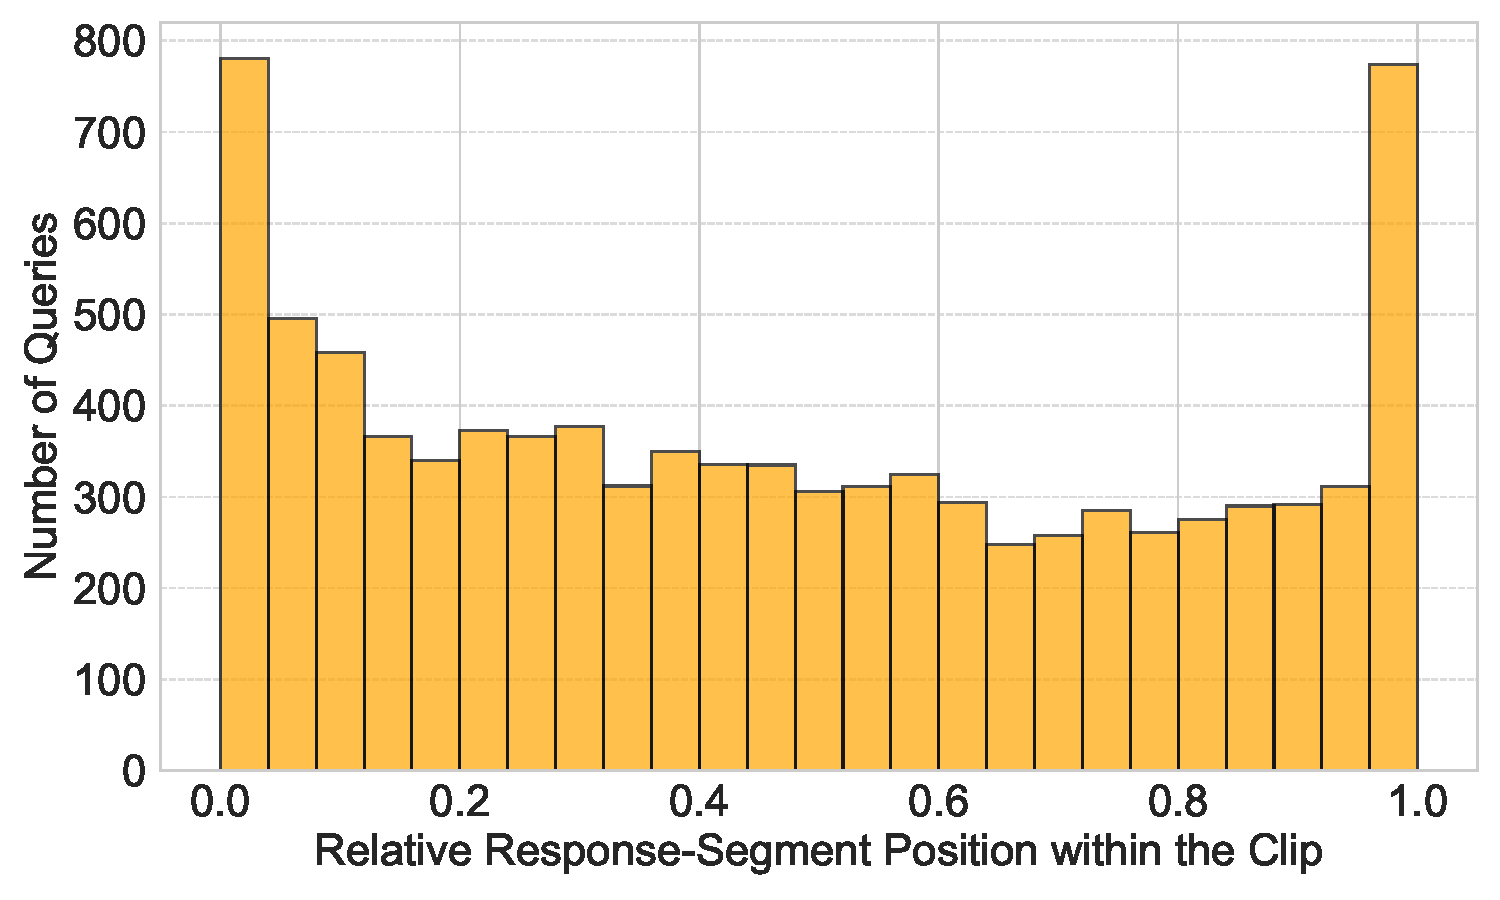
\includegraphics[width=1\linewidth]{images/RelativeSegmentPosition_large_font.pdf}
    \caption{Number of queries by relative Response-Segment position within their clip.}
    \label{fig:6}
\end{figure}

Considering the analysis of ego4d.json, instead, we examined only a subset of the Ego4D dataset, focusing on the videos also present in nlq\_train.json. The dataset thus obtained includes 136 distinct scenarios, as the whole ego4d.json, and this highlights once again how varied and diverse the NLQ annotations dataset is.\\
In particular, we found that the most frequent scenarios are Cooking, Cleaning/Laundry, Car mechanic, and Indoor navigation (walking), which are, not by coincidence, situations where it is easier to identify various non-repetitive actions and objects. Due to this favorable nature, more space has been dedicated to them within the dataset.


\section{Methodology}
In this section, we first present the architectures used to handle the NLQ task, then the process to generate the queries using Gemma, and finally we describe the pre-training and fine-tuning steps.

\subsection{Architectures}
To tackle the NLQ challenge we used the models \textit{VLSBase} and \textit{VSLNet} \cite{zhang2020spanbasedlocalizingnetworknatural}, with the latter being an extension of the former and characterized by superior performance thanks to an effective Query-Guided Highlighting (QGH) strategy.\\
Differently from the original paper, we did not obtain the visual features with a 3D ConvNet, but we used pre-extracted features from Omnivore and EgoVLP.
To encode the queries we employed BERT for most of the steps, but we considered also GloVe as an alternative.\\
In VSLBase, since addressing an NLVL task requires jointly handling textual and visual features and uncovering the interconnections between them, both features are projected into a shared space using two linear layers, unifying the dimensions of the vectors. A single and shared Feature Encoder encodes these features and the Context-Query Attention (CQA) component captures cross-modal interactions. The CQA computes the similarity scores and the attention weights that help to determine how closely related is each visual feature to the relative query feature, refining the representations. Finally, the Conditioned Span Predictor predicts the start and end boundaries of the answer span. \\
VSLNet builds on top of this structure by adding the QGH. Specifically, it considers the target moment, beginning with $a_s$ and ending with $a_e$, as the \textit{foreground} and the rest as the \textit{background}. QGH extends the boundaries of the foreground to include its preceding and following video content, where the extension ratio is controlled by a hyperparameter $\alpha$.
By assigning a value of \(1\) to visual features in the foreground and \(0\) to those in the background, QGH becomes a binary classification module that estimates the probability that a visual feature is part of the foreground or background.\\
This last strategy has two significant advantages: firstly, the expanded region offers additional context for identifying the answer span thanks to the continuous nature of video content. Secondly, the highlighted region enables the network to concentrate on subtle differences between video frames, since the search space is at this point significantly smaller compared to the entire video.

 \subsection{Tests}
Before going into detail about the query generation step, we will briefly mention here a few tests we conducted starting from the reference model VSLNet and analyzing the effects and results of not employing the query-guided highlighter, using different visual features, changing the text encoder. \\
We started by training for 10 epochs both VSLBase and VSLNet twice, first with the pre-extracted visual features from Omnivore, then from EgoVLP, while using the same textual NLQ annotations.\\
In particular, we utilized pre-trained features extracted using temporal windows of 32 frames and temporal stride 16, in line with the official Ego4D pre-extracted features.
After training, we evaluated the 4 different models on the validation set and on the test set.\\
Subsequently, we implemented a small variation of VSLNet by replacing the text encoder \textit{BERT} with \textit{GloVe}, whose properties have already been outlined in the previous section.\\


\subsection{Query generation}
We created a new and more diverse set of queries related to the entire Ego4D dataset using the available narrations. This data augmentation aims to expose the VSLNet model to a wider range of scenarios during a pre-training phase, before moving on to fine-tuning and using the original, specific training set of NLQ annotations.\\ 
The additional queries for pre-training were generated using the \textit{Gemma-2b-it-V2} LLM which was instructed to produce new questions starting from a set of randomly sampled consecutive \textit{narrations} (coming from the narration.json file). These are nothing more than textual annotations covering all Ego4D videos, briefly describing the activity the user is performing at a given moment.

\subsubsection{Sampling groups of narrations}
To sample the narrations, we started excluding the videos of the Ego4D dataset included in the test and validation sets of the NLQ task to avoid a data leak to the training set.\\ 
For simplicity we selected one group of consecutive narrations for each annotation uid, a field with similar properties to clip uid, which is not available in the narrations file, intending to generate new queries covering the selected set of narrations.\\
Samples of \textit{n} consecutive narrations were taken by randomly selecting the first narration, ensuring that the sample did not present any narration with a "status" field different from "complete" and avoiding those containing the word "unsure" inside the "narration\_text" attribute. This operation was performed to facilitate the job of the LLM, which, not receiving incomplete narrations, could provide better quality queries. Additionally, since the pre-trained visual features are based on the clip reference system, sets sharing the same annotation uid but that were not entirely contained within a single clip were also excluded from the sampling.  \\
An important step was the definition of the extremes of the interval of the sample and consequently the ground truth of the future annotations. The input file presents only the starting time at which each narration is performed, not an interval. From this “limitation” derived our idea to take consecutive narrations and use the timestamps of the first narration in the sample and the one after the last as borders for the response.\\
Since we already had a good level of variety given by both the free form of the queries generated by the LLM and especially by leveraging a large and diverse set of videos and scenarios (while the annotations of the train set of the NLQ task follow specific templates and cover just a subset of the Ego4D dataset), we aimed to match as close as possible the distribution of the ground truth segment durations of the fine-tuning dataset. In this way, we tried to limit the domain gap between pre-training and fine-tuning datasets. Following this idea, we also avoided creating annotations with very wide response intervals from which the model would have potentially learnt less transferable concepts. We were able to regulate the ground truth duration by modifying the cardinality of the sample of narrations \textit{n}: the more consecutive narrations the wider the interval.\\
We therefore conducted a brief analysis of the response segment length in nlq\_train.json, finding an average duration of approximately 9.67 seconds. We then observed the average duration covered by the samples of narrations as \textit{n} varied. Starting from \textit{n} = 2, the average duration was 13.81 seconds, while, for \textit{n} = 3, it was 20.00 seconds, both comparable with nlq\_train.json. 
Additionally, we also considered the configuration starting from \textit{n} = 5 narrations, which had an average duration of the response interval considerably higher than the original NLQ set (about 31.64 seconds), to be able to analyze the impact of different lengths of ground truth on the results.
To have a fair comparison among the three configurations and at the same time a number of queries similar to the one of the original annotations set, we decided to produce in all three cases 8500 queries. This value was obtained empirically by checking that all three configurations were always able to produce a quantity of queries slightly greater than this value, which is close enough to the number of queries of nlq\_train.json. To achieve this, we instructed the LLM to provide, respectively, \textit{m} = 2, 2 and 3 queries.

\subsubsection{LLM prompt}
To obtain a good level of quality for the queries generated by the LLM, we manually tested different prompts and output lengths. The three main prompts that we tested are:

\begin{enumerate}
    \item[A)] "You are trying to help humans to augment their memory. To achieve this goal some annotators have watched several videos about people performing different actions in various scenarios, writing down, step by step, short narrations describing in a few words what is happening in the video and the time at which these actions take place. You are requested to generate 2 simple queries that a person could answer just by looking at the video segments corresponding to these narrations:" + formatted\_narrations[i] + " To do so follow these rules:  - do not include the answer in the question - avoid introductions, report just the text of the queries one per line"
    \item[B)] "Generate two short simple queries that a person could answer looking at the video corresponding to these narrations: "+ formatted\_narrations[i]+ "\textbackslash nIn your answer report just the queries one per line"
    \item[C)] "Generate two questions mixing the information of these sentences: \textbackslash""+ formatted\_narrations[i]+ "\textbackslash"\textbackslash nIn your answer write only two lines with a question each"
\end{enumerate}

Running several tests we were able to notice that the simpler the prompt the better-quality were the queries obtained. Here is an example: \\ \\
Narration:  "C fixes the camera.  C walks in the supermarket.  C picks the shopping basket"\\
$\bullet$ Result prompt A: ['What is the person doing at 2 minutes and 40 seconds into the video?'] \\
$\bullet$ Result prompt B: [‘What is the action that C does in the video?’, ‘What does C do in the supermarket?’] \\
$\bullet$ Result prompt C: ['Where did C fix the camera?', 'What was C doing while walking into the supermarket?'] \\\\
This behavior is probably related to the fact that we used a light version of Gemma, which, not being as powerful as the latest LLMs, struggled with long and detailed prompts. For this reason, in the end, we employed the prompt C.\\
To decide the output length in tokens of the model, we operated a trade-off between the speed of generation and the number of queries generated.  Different lengths of output did not have a significant influence on the quality of the queries, but in our tests we were able to appreciate how the longer the output the longer was the generation process. On the other hand, however, when we adopted a too short output length, the LLM was often not able to terminate the queries, which had to be filtered out because incomplete, reducing the final number of producible annotations. For these reasons, we sought the shortest output with a negligible number of incomplete queries which resulted in being 20 tokens for each query generated.

\subsection{Pre-training and fine-tuning}
We will now discuss how we managed the pre-training and fine-tuning phases. In both circumstances, we fine-tuned on the original NLQ annotations dataset for 10 epochs to have a direct comparison with the results of VSLNet without pre-training. During pre-training VSLNet was trained on the 8500 newly generated queries, while for the fine-tuning we trained the model on the nlq\_train.json set, testing two different versions of fine-tuning. Specifically, we experimented firstly by updating the parameters of all layers and secondly by freezing some layers. In the latter case, the achievable results will indicate the generality of the concepts learnt during pre-training.\\
In the second version, we decided to freeze until the CQA block, leaving the remaining modules trainable because the CQ-Attention module captures cross-modal interactions, which are low-level concepts that can be effectively learned during pre-training. In contrast, the QGH module and the Conditioned Predictor are more specifically tailored to the NLQ task and, thus, we kept them trainable during fine-tuning to better adapt to the specific job.

In \cref{{seq:results}}, we will present the results obtained for all the different settings: varying \textit{n}, \textit{m} and the type of fine-tuning applied.



\section{Experimental Section - Results}
\label{seq:results}
In this section we will present all the results obtained from the tests we conducted and described in the previous sections.
\subsection{Evaluation metrics}
As evaluation metric, we adopted “recall@k, IoU= t”, following the video-language grounding literature. This metric denotes the percentage of times where at least one of the top-k predicted moments has an intersection-over-union (IoU) with the ground truth greater or equal to t. In our case, we report the results for k = {1,5} and t = {0.3, 0.5}.
\subsection{Baselines}
Our goal is to evaluate the effect of our extension combined with existing methods present in the literature. For this reason, we first evaluated the baselines for the task, to be able to have a measure of comparison for our results. \\
In \cref{tab:omn_egovlp_vslnet_vslbase}, we report the results we obtained on the validation and test set comparing VSLNet and VSLBase which are given as input the visual features generated by Slowfast (official NLQ baseline provided by Ego4D, see details in \cite{grauman2022ego4d}), Omnivore and EgoVLP. 
As expected and explained in \cite{zhang2020spanbasedlocalizingnetworknatural}, VSLNet, thanks to the query-guided highlighter module, performs better than VSLBase across all metrics. The performance gap is more evident for the visual features obtained with EgoVLP. \\
Regarding the visual feature extractors, VSLNet reaches better results receiving the video features from EgoVLP than from Omnivore or Slowfast. This is due to the fact that, while Omnivore is a general-purpose model designed to handle a large variety of visual tasks and Slowfast is primarily designed for general video action recognition, EgoVLP, instead, is specifically designed for egocentric video-language pre-training.


\begin{table}[]
    \centering
    \small
    \setlength{\tabcolsep}{4pt}
    \begin{tabular}{|c|c|c|c|c|c|}
        \hline
        \multirow{Vis. Feat} & \multirow{Model} & \multicolumn{2}{c|}{IoU = 0.3 (\%)} & \multicolumn{2}{c|}{IoU = 0.5 (\%)} \\  \cline{3-6} 
        &  & r@1 & r@5 & r@1 & r@5 \\ \hline  
        \multicolumn{6}{|c|}{Validation} \\ 
        \hline SlowFast & VSLNet & 5.45 & 10.74 & 3.12 & 6.63 \\ \hline 
        \multirow{Omnivore} & VSLNet & 6.22 & 13.19 & 3.54 & 8.18 \\ \cline{2-6} 
        & VSLBase & 5.58 & 12.13 & 2.76 & 7.77 \\ \hline
        \multirow{EgoVLP} & VSLNet & \textbf{7.90} & \textbf{15.75} & \textbf{5.06} &  \textbf{10.33} \\ \cline{2-6} 
        & VSLBase & 5.63 & 12.70 & 3.36 & 8.26 \\ \hline
        \multicolumn{6}{|c|}{Test} \\ 
        \hline      
        SlowFast & VSLNet & 5.47 & 11.21 & 2.80 & 6.57 \\ \hline 
        \multirow{Omnivore} & VSLNet & 6.56 & 11.26 & 3.67 & 6.89 \\ \cline{2-6} 
        & VSLBase & 6.54 & 10.96 & 3.84 & 6.61 \\ \hline
        \multirow{EgoVLP} & VSLNet & \textbf{8.66} & \textbf{13.68} & \textbf{5.26} & \textbf{9.09} \\ \cline{2-6} 
        & VSLBase & 5.64 & 10.66 & 3.47 & 6.81 \\ \hline
    \end{tabular}
    \caption{Results obtained by VSLNet and VSLBase models, compared to the baseline using Slowfast provided by Ego4D, trained on different sets of visual features and with BERT.}
    \label{tab:omn_egovlp_vslnet_vslbase}
\end{table}

\subsection{Variation of Text Encoder}
\cref{tab:glove_bert} contains the results obtained with two different text encoders: BERT and GloVe. As clearly shown in the table BERT significantly outperforms GloVe across all metrics, leveraging contextual embeddings, bidirectional training, and a sophisticated transformer architecture exploiting self-attention mechanisms. GloVe, on the other hand, uses static embeddings and is more focused on word frequency and co-occurrence patterns than on the actual semantic meaning in the context. However, thanks to its simpler approach, GloVe is faster than BERT: measuring the elapsed time for the training with the two configurations of VSLNet we obtained 10 minutes and 23 seconds using BERT and 9 minutes and 32 seconds employing GloVe. Nonetheless, considering the total duration of the process, the advantage in time is not that significant to lead us to choose GloVe over the better-performing BERT.\\
For the final step of the analysis, we adopted the best performing configuration: VLSNet with EgoVLP features and BERT text encoder.

\begin{table}[]
    \centering
    \small
    \setlength{\tabcolsep}{4pt}
    \begin{tabular}{|c|c|c|c|c|}
        \hline
        \multirow{Configuration} & \multicolumn{2}{c|}{IoU = 0.3 (\%)} & \multicolumn{2}{c|}{IoU = 0.5 (\%)} \\  \cline{2-5} 
        & r@1 & r@5 & r@1 & r@5 \\ \hline
        \multicolumn{5}{|c|}{Validation} \\ 
        \hline     
        VSLNet \& BERT & \textbf{6.22} & \textbf{13.19} & \textbf{3.54} & \textbf{8.18} \\ \hline
        VSLNet \& Glove & 3.05 &  8.36 & 1.21 & 4.34 \\ \hline
        \multicolumn{5}{|c|}{Test} \\  
        \hline     
        VSLNet \& BERT & \textbf{6.56} & \textbf{11.26} & \textbf{3.67} & \textbf{6.89} \\ \hline
        VSLNet \& Glove & 3.54 & 7.21 & 1.72 & 4.02 \\ 
        \hline     
    \end{tabular}
    \caption{Results obtained by VSLNet model, trained on the Omnivore visual features, with BERT and Glove as text encoders, on the validation set and the test set.}
    \label{tab:glove_bert}
\end{table}


\subsection{Automatic queries generation with LLM}
In this final section we will present the results obtained by pre-training the VSLNet on a set of annotations containing the queries automatically generated with Gemma from the dense narrations provided by Ego4D. They are summarized in \cref{tab:results_extension}.\\
As described in the methodological section, once we had pre-trained the VSLNet using the new set of annotations, we conducted two experiments: in one case we fine-tuned all layers of our model, in the other one we froze the model’s parameters until the context query attention layer. \\
Even if the number of epochs for which we pre-trained our model was limited (only 10, due to limited resources), the model is learning from the generated queries, as shown by the recall rates after the pre-training phase in \cref{tab:results_pretraining}. Our approach, when we let then all layers free and fine-tune the model for 10 epochs, reaches better results across all metrics, outperforming the baselines. \\
These results confirm our hypotheses: by exposing the model to a wider range of linguistic structures and visual contexts it is possible to enhance its performance.\\
The results also highlight the impact of different fine-tuning strategies: fine-tuning all layers after pre-training shows better performance than freezing the initial layers and only updating the last two. This indicates that the model benefits more from a holistic adjustment to the new task-specific data. When only the last few layers are fine-tuned, a significant part of the model remains fixed with its general pre-training knowledge. In this case, not being able to adjust the parameters of the first layers to better align with the new task leads to suboptimal performance, probably because the gap between pre-training and fine-tuning datasets is significant, since in the first case we are dealing with free-form automatically generated queries. \\
Another possible explanation is that our limited number of epochs and queries, due to the few resources, are not sufficient to fully capture the knowledge and features that LLM-generated queries and videos can provide, on top of which fine-tuning only the last layers could be more beneficial.  \\
For what concerns the different experiments conducted varying the number of narrations from which we generated the queries, as shown in \cref{tab:results_extension}, no clear difference is evident in the results. This suggests that pre-training the model using ground truths of different lengths does not have a significant impact at fine-tuning time (for the mechanism of extraction of narrations and the way in which we compute the relative ground truth, on average the amplitude of the interval to identify increases when the number of narrations increases). \\
The most significant limitation of this approach is probably the inability to assess the quality of the generated queries automatically. While the set of annotations provided by Ego4D is generated manually, following specific indications and rules, generating queries with an LLM can provide unpredictable results, especially if, like in our case, a light version is used. However, even with a “smarter” LLM, capable of always generating sensible and pertinent queries, some problems still arise: for instance there is no way to instruct the LLM, which just receives few narrations, to avoid generating queries whose answer could be contained also in another segment of the video, situation that is specifically avoided in the case of the manual annotations.       


\begin{table}[]
\centering
\small 
\setlength{\tabcolsep}{4pt}
    \begin{tabular}{|c|c|c|c|c|}
        \hline
        \multirow{Pre-training} & \multicolumn{2}{c|}{IoU = 0.3 (\%)} & \multicolumn{2}{c|}{IoU = 0.5 (\%)} \\  \cline{2-5} 
        & r@1 & r@5 & r@1 & r@5 \\ \hline         
        Before & 1.21 & 2.89 & 0.44  & 1.21 \\ \cline{1-5} 
        \hline          
        After &  2.84 & 6.22 & 1.45  & 3.69 \\ \hline
    \end{tabular}
    \caption{Results obtained on the validation set by the VSLNet model with BERT and EgoVLP features, before and after pre-training on different sets of two new queries generated by \textit{Gemma} from samples of three consecutive narrations.}
    \label{tab:results_pretraining}
\end{table}


\begin{table}[]
\centering
\small 
\setlength{\tabcolsep}{4pt}
    \begin{tabular}{|c|c|c|c|c|}
        \hline
        \multirow{Configuration} & \multicolumn{2}{c|}{IoU = 0.3 (\%)} & \multicolumn{2}{c|}{IoU = 0.5 (\%)} \\  \cline{2-5} 
        & r@1 & r@5 & r@1 & r@5 \\ \hline
        
        Best baseline & 7.90 & 15.75 & 5.06 &  10.33 \\ \hline
        
        \multicolumn{5}{|c|}{Updating all layers} \\ 
        \hline     
       \textit{n}=2, \textit{m}=2 & 8.80 & \textbf{17.27} & \textbf{5.50}  & 11.20 \\ \cline{1-5} \textit{n}=3, \textit{m}=2 
      & 8.65 & \textbf{17.27} & 5.06 & 11.38 \\ \cline{1-5}
      \textit{n}=5, \textit{m}=3 & \textbf{9.09} & 16.88 & 5.32 & \textbf{11.49} \\ \hline        
        \multicolumn{5}{|c|}{Freezing some layers} \\ 
        \hline
       \textit{n}=2, \textit{m}=2 & \textbf{4.03} & \textbf{9.65} & 2.48 & 5.83 \\ \cline{1-5} \textit{n}=3, \textit{m}=2 
      & 3.87 & 9.53 & 2.01 & \textbf{5.96} \\ \cline{1-5}
      \textit{n}=5, \textit{m}=3 & 3.98 & 9.16 & \textbf{2.56} &  5.65 \\ \hline
    \end{tabular}
    \caption{Results obtained on the validation set by the VSLNet model with BERT and EgoVLP features, pre-trained on different sets of \textit{m} new queries generated by \textit{Gemma} from samples of \textit{n} consecutive narrations, and fine-tuned on the original NLQ annotations. In the second part, the results are obtained freezing the first layers and updating only the last 2 layers.}
    \label{tab:results_extension}
\end{table}




\section{Conclusions}
To summarize, we focused on the Episodic Memory benchmark and used state-of-the-art models and new methods for data augmentation and pre-training.\\
First, we compared the performance of VSLNet and VSLBase models using two sets of visual features: Omnivore and EgoVLP. We found that VSLNet, especially with EgoVLP features, consistently outperformed VSLBase across all metrics.\\
Next, we tested different text encoders on VSLNet: BERT performed considerably better than GloVe, showing the benefits of contextual embeddings for understanding natural language queries.\\
To further improve the results, we created an automatic query generation process using the \textit{Gemma-2b-it-V2} large language model. Pre-training VSLNet on these generated queries led to noticeable improvements, especially when we fine-tuned all layers of the model. This confirmed that exposing the model to a wider range of language structures enhances its performance.\\
Finally, we observed that different strategies for freezing model layers during fine-tuning have different impacts on performance.  Fine-tuning all layers after pre-training gave better results than freezing the initial layers, indicating that leaving the model free to adapt to new task-specific data is important for optimal performance in our case.\\
Overall, our findings suggest that a combination of pre-extracted visual features, contextual text embeddings, and extensive pre-training on automatically generated queries can significantly improve the performance of our models on NLVL tasks in egocentric video datasets.\\
Future work may explore further optimization of the query generation process and fine-tuning strategies to continue improving first-person video understanding without the restrictions on the number of generated queries and pre-training epochs imposed by our limited resources.\\
Code available at: \href{https://github.com/Cucchi01/episodic-memory/tree/nlq_fixes_and_fp16_support}{https://github.com/Cucchi01/episodic-memory/tree/nlq\_fixes\_and\_fp16\_support}.

%-------------------------------------------------------------------------

%%%%%%%%% REFERENCES
{\small
\bibliographystyle{ieee_fullname}
\bibliography{egbib}
}

\end{document}
